\begin{frame}
\frametitle{Evaluación}

\begin{itemize}
	\item<1-> Se han procedido a realizar diferentes pruebas con distintas variables.
	
	\vspace{1em}
	
	\item<2-> Por ejemplo, definiendo distintos tamaños de escenarios.
\end{itemize}

\vspace{1em}

\pause[3]

\centering
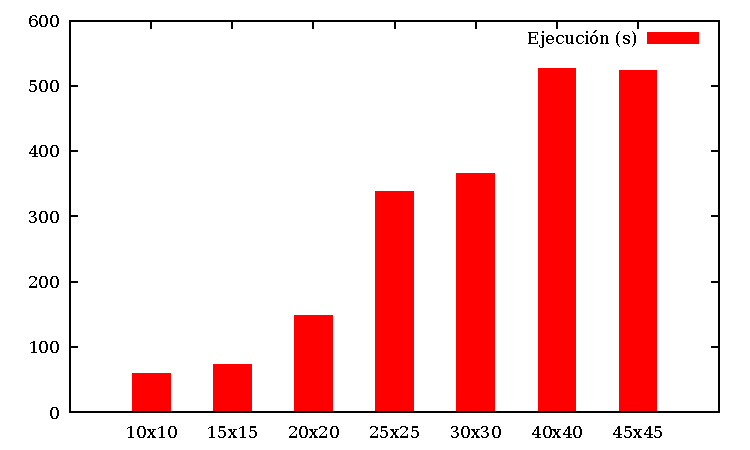
\includegraphics[width=0.8\textwidth]{images/map-size.pdf}

\end{frame}

\begin{frame}
\frametitle{Evaluación}

\begin{itemize}
	\item<1-> Modificado porcentajes de terreno con tierra y tamaño de biomas.
	
	\vspace{0.5em}
	
	\item<2-> Se observa la  misma tendencia que en la primera prueba.
\end{itemize}

\pause[2]

\begin{table}[!h]
	\centering
	\begin{tabular}{cc|cccccc}
		& & \multicolumn{6}{c}{Tamaño de biomas} \\
		& & 10\% & 15\% & 20\% & 25\% & 30\% & 35\% \\
		\hline
		\parbox[t]{2mm}{\multirow{12}{*}{\rotatebox[origin=c]{90}{Tamaño de tierra}}} & 10\% & 42 s & 41 s & 35 s & 88 s & 117 s & 214 s \\
		& 15\% & 41 s & 37 s & 36 s & 88 s & 133 s & 247 s \\
		& 20\% & 37 s & 43 s & 37 s & 105 s & 123 s & 224 s \\
		& 25\% & 29 s & 51 s & 43 s & 92 s & 123 s & 220 s \\
		& 30\% & 42 s & 43 s & 138 s & 95 s & - & - \\
		& 35\% & 41 s & 40 s & 38 s & 90 s & - & 241 s \\
		& 40\% & 43 s & 46 s & 36 s & -  & - & 217 s  \\
		& 45\% & 69 s & 49 s & 36 s & 737 s & - & 220 s \\
		& 50\% & 100 s & - & 1064 s & - & - & - \\
		& 55\% & 55 s & 956 s & - & - & - & - \\
		& 60\% & 164 s & 740 s & - & - & - & - \\
		& 65\% & 97 s & 838 s & - & - & - & - \\
		\hline
	\end{tabular}
\end{table}

\end{frame}